
%(BEGIN_QUESTION)
% Copyright 2012, Tony R. Kuphaldt, released under the Creative Commons Attribution License (v 1.0)
% This means you may do almost anything with this work of mine, so long as you give me proper credit

A 15 kV three-phase alternator needs to have its windings connected properly to prepare it to send power to a ``bus'' shared by other alternators in a power plant:

$$\includegraphics[width=15.5cm]{i01043x01.eps}$$

Each phase winding on the alternator is rated at 15 kV.  The rotor winding is rated at 220 VDC.  Sketch all necessary connections to make this alternator work as intended.

\underbar{file i01043}
%(END_QUESTION)





%(BEGIN_ANSWER)

This is one possible solution, but not the only one:

$$\includegraphics[width=15.5cm]{i01043x02.eps}$$

%(END_ANSWER)





%(BEGIN_NOTES)


%INDEX% Electronics review: 3-phase electrical power 
%INDEX% Pictorial circuit review (3-phase alternator connections)

%(END_NOTES)

